\documentclass[a4paper]{article}
\usepackage[14pt]{extsizes}
\usepackage[utf8]{inputenc}
\usepackage[ukrainian]{babel}
\usepackage{setspace,amsmath}
\usepackage[left=20mm, top=15mm, right=15mm, bottom=15mm, nohead, footskip=10mm]{geometry} % настройки полей документа
\usepackage{tocloft}
\usepackage{indentfirst}
\usepackage{amsfonts}
\usepackage{wrapfig}

\usepackage{graphicx}
\graphicspath{}
\DeclareGraphicsExtensions{.pdf,.png,.jpg}

\usepackage{hyperref}
\hypersetup{
  colorlinks=false,
  linkcolor=blue,
  filecolor=magenta,      
  urlcolor=cyan,
  pdftitle={Розподілені алоритми пошуку рівноваги Неша}
}

\makeindex

\begin{document}

\thispagestyle{empty}

\begin{center}
Міністерство освіти та науки України\\
Київський національний університет імені Тараса Шевченка\\
Факультет комп’ютерних наук та кібернетики\\
Кафедра обчислювальної математики\\

\vfill

\huge{\textbf{КУРСОВА РОБОТА}}\\
\large{на тему:}\\
\LARGE{\textbf{Розподiленi алгоритми пошуку рiвноваги Неша}}\\

\end{center}
\vfill

\begin{flushleft}
\quad\quad\quad\quad\quad\quad\quad\quad\quad\quad\quad\quad\quad\quad\quad\quad\quad\quad\quad{Виконав студент III курсу}\\
\quad\quad\quad\quad\quad\quad\quad\quad\quad\quad\quad\quad\quad\quad\quad\quad\quad\quad\quad{групи ОМ-3}\\
\quad\quad\quad\quad\quad\quad\quad\quad\quad\quad\quad\quad\quad\quad\quad\quad\quad\quad\quadПівень Денис Миколайович\\
\quad\quad\quad\quad\quad\quad\quad\quad\quad\quad\quad\quad\quad\quad\quad\quad\quad\quad\quadКерівник курсової роботи\\
\quad\quad\quad\quad\quad\quad\quad\quad\quad\quad\quad\quad\quad\quad\quad\quad\quad\quad\quadдоктор фізико-математичних наук\\
\quad\quad\quad\quad\quad\quad\quad\quad\quad\quad\quad\quad\quad\quad\quad\quad\quad\quad\quadпрофесор кафедри обчислювальної\\
\quad\quad\quad\quad\quad\quad\quad\quad\quad\quad\quad\quad\quad\quad\quad\quad\quad\quad\quadматематики\\
\quad\quad\quad\quad\quad\quad\quad\quad\quad\quad\quad\quad\quad\quad\quad\quad\quad\quad\quadСеменов Володимир Вікторович\\
\end{flushleft}

\vfill

\centerline{Київ – 2021}
\clearpage

\renewcommand\cftsecdotsep{\cftdot}
\cftsetpnumwidth{9pt}
\tableofcontents
\clearpage

\section{Вступ}
Протягом життя ми постійно взаємодіємо з іншими людьми. Маленькі діти, намагаючись добитися того, щоб батьки купили вподобану цукерку, часто шантажують батьків своїми слізьми. Приймаючи рішення заплакати, дитина ризикує — він не знає, як будуть поводитися тато з мамою. У трохи більш дорослому віці абітурієнти, які вибирають виш, приймають складне рішення в тому, до яких університетів подати документи. Помилка може коштувати дорого: при неправильній стратегії можна опинитися в слабкому університеті або взагалі залишитися без заповітного студентського квитка. Закінчивши виш, юнаки й дівчата починають шукати роботу. Перед інтерв'ю з роботодавцем вони переглядають статті в інтернеті в тому, що можна і чого не можна говорити на інтерв'ю, — вони намагаються знайти найкращу стратегію своєї поведінки, виходячи з очікувань компанії, в яку вони влаштовуються. Всі ці ситуації об'єднує те, що рішення, які приймають люди, впливають на інших. Пошук найкращої стратегії є не тривіальною задачею, як для дитини, так і для дорослого. На жаль не всі діють за принципами теорії прийняття рішень, теорії ігор чи просто аналітично розв'язують поставлену перед ними проблему

На мій погляд, найбільший вплив проблема пошуку оптимального рушення відіграє в економіці. На сьогодні, згідно з економічною теорією, конкурентна рівновага є оптимальним станом економіки, і відхилення від нього пов'язано зі зниження її ефективності. Одна з можливих причин цього відхилення — зміна ціни товару в результаті дій виробника або споживача товару, який контролює значну частку в загальному обсязі продажів. Велика частина реальних ринкових продажів олігополії. В той час, як окремий споживач не має ринкової влади і його вплив у загальному обсязі продажів складає соті відсотка, найбільший виробник на таких ринках забезпечує не менше 10\% від загального споживання. Дослідження математичних моделей і оцінка очікуваного відхилення від стану конкурентної рівноваги для різних типів олігополії становлять великий інтерес. Типовим підходом до кількісної характеристики умов досконалої конкуренції та до оцінки очікуваного відхилення є порівняння конкурентної рівноваги з рішенням гри, яка описує олігополістичну конкуренцію.

Метою даної курсової роботи є дослідження постановки математичної моделі заданої проблеми та алгоритмів пошуку її оптимального рішення. Також дослідження думок людей під час прийняття рішень, та донесення базової інформації про дисципліну, якої звісно буде недостатньо для повного розуміння теорії ігор, але цілком вистачить для оглядового сприйняття. 


\clearpage
\section{Джон Неш}
Джон Форбс Неш молодший (англ. John Forbes Nash, Jr.; 13 червня 1928, Блуфілд, США — 23 травня 2015, Монро, США) — американський математик, що зробив значний внесок у розвиток теорії ігор та диференціальної геометрії. Лауреат Нобелівської премії з економіки 1994 року (разом з Райнгардом Зельтеном і Джоном Харсані), Абелівської премії 2015 року (разом з Луїсом Ніренбергом).

Поза професійними колами відомий тим, що захворів на шизофренію, від якої по тривалім часі спонтанно одужав і повернувся до нормального життя. Доля Джона Неша-молодшого описана в біографічному романі Сильвії Назар \textit{«Блискучий розум»}, за яким знято оскароносний фільм \textit{«Ігри розуму»}.

Першим суспільно вагомим внеском Джона Неша була настільна логічна гра гекс. Він вигадав її 1949 року під час навчання в аспірантурі Принстонського університету. Хоча гру з аналогічними правилами у 1942 році запропонував данець Піт Гейн, однак Неш не знав про його винахід і свою ідею подав цілком незалежно. Нешів товариш Девід Ґейл придумав оформлення і зайнявся комерційним просуванням гри у винагороду за відсоток від продажів. Хоча в університетських колах гру називали на честь автора \textit{«нешем»} або \textit{«джоном»}, у комерційному виробництві поширилась назва, запропонована Ґейлом (від гексагональної форми ігрових чарунок). У середині 1950—х років гекс випускала фірма \textit{«Паркер бразерс»} і деякий час гра була популярна у досить широких колах.

У Принстоні Джон Неш ознайомився з роботою Джона фон Неймана та Оскара Морґенштерна, в якій автори запропонували математичну модель для визначення оптимальних рішень в умовах конфлікту. Почавши з дослідження ігор з повною інформацією (наприклад, шах чи хрестиків-нуликів), в яких кожен з гравців від початку знає про ресурси та становище супротивника, економісти перейшли до аналізу складніших ігор з неповною інформацією, в яких гравцям заздалегідь невідомі можливості супротивника. До останнього типу можна було віднести як покер, так і масштабніші ситуації: економічні санкції, війни чи розлучення. Запропонована фон Нейманом і Морґенштерном теорія ігор давала можливість чітко визначити стратегію прийняття рішень, однак вона стосувалася лише ігор з нульовою сумою, тобто таких, в яких перемога однієї сторони означає повну поразку іншої.

Упродовж 1950-1953 років Неш опублікував чотири революційні роботи, в яких представив глибокий аналіз ігор з ненульовою сумою, — особливого класу ігор, в яких виграш одного учасника не обов'язково означає програш іншого. Джон Неш взяв до уваги, що в реальному житті ситуації непримиренного антагонізму трапляються рідко, і частіше доводиться приймати рішення в умовах, коли учасники конфлікту зацікавленні у компромісі. Прикладом такої гри є переговори про збільшення зарплати між профспілкою і керівництвом компанії. Ця ситуація може завершитися або тривалим страйком, в якому постраждають обидві сторони, або взаємовигідною угодою. Неш зумів розгледіти нове обличчя конкуренції, моделюючи ситуацію, яка згодом отримала назву \textit{«рівновага Неша»} або \textit{«некооперативна рівновага»}, при якій обидві сторони використовують ідеальну стратегію, що й приводить до створення стійкої рівноваги. Гравцям вигідно зберігати цю рівновагу, оскільки будь—яка зміна тільки погіршить їхнє положення, однак відповідна стратегія може бути програшною для всіх, і тоді більшого виграшу можна досягти тільки при кооперуванні. Один з його прикладів — задача про оборудку — став хрестоматійною класикою економічної теорії.

На момент публікацій, роботи Джона Неша не зацікавили математиків і були сприйняті з обережним оптимізмом економістами. Однак з часом збільшувалось число галузей, в яких рівновага Неша виявилась практичною концепцією. Окрім математичного аналізу й економіки удосконалену теорію ігор почали застосовувати щодо менеджменту та, навіть, еволюційної біології. Засади теорії ігор, застосовані в умовах фондового ринку чи державних аукціонів принесли лише тільки уряду США мільярдні прибутки, при тому, що розвитком теорії займалися дослідники й інших країн світу.

\section{Теорія ігор}
Як математична дисципліна, теорія ігор зародилась одночасно з теорією ймовірностей в XVII столітті, але протягом майже 300 років практично не розвивалась. Першою істотною роботою з теорії ігор слід вважати статтю Дж.~фон Неймана \textit{«До теорії стратегічних ігор»(1928)}, а з виходом у світ монографії американських математиків Дж.~фон Неймана та О. Морґенштерна \textit{«Теорія ігор і економічна поведінка»(1944)}\cite{Neyman}, теорія ігор сформувалась як самостійна математична дисципліна. На відміну від інших галузей математики, які мають переважно фізичне, або фізико-технологічне походження, теорія ігор із самого початку свого розвитку була направлена на розв'язання задач, які виникають в економіці (а саме в конкурентній економіці).

Надалі, ідеї, методи та результати теорії ігор почали застосовувати в інших галузях знань, які мають справу з конфліктами: у військовій справі, в питаннях моралі, при вивченні масової поведінки індивідів, які мають різні інтереси (наприклад, в питаннях міграції населення, або при розгляді біологічної боротьби за існування). Теоретико-ігрові методи прийняття оптимальних рішень в умовах невизначеності можуть мати широке застосування в медицині, в економічному і соціальному плануванні та прогнозуванні, в ряді питань науки та техніки. Іноді теорію ігор відносять до математичного апарату кібернетики, або теорії дослідження операцій.

\subsection{Класифікація ігор}
\subsubsection*{Кооперативні або некооперативні}
Гра називається кооперативною, якщо гравці можуть об'єднуватися в групи, взявши на себе деякі зобов'язання перед іншими гравцями та координуючи свої дії. Цим вона відрізняється від некооперативних ігор, в яких кожен зобов'язаний грати за себе. Некооперативні ігри описують ситуації в найменших подробицях і видають більш точні результати. Кооперативні розглядають процес гри в цілому. Гібридні ігри включають елементи кооперативних та некооперативних ігор. Наприклад, гравці можуть створювати групи, але гра буде проводитись в некооперативному стилі. Це означає, що кожен гравець буде переслідувати інтереси своєї групи, разом з тим досягти особистої вигоди.

\subsubsection*{Симетрична та антисиметрична гра}
Симетрична гра буде симетричною тоді, коли відповідні стратегії у гравців будуть рівними, тобто вони матимуть однакові платежі. Інакше кажучи, якщо гравці поміняються місцями й при цьому їх виграші за ті ж самі ходи не зміняться.

\subsubsection*{З нульовою і ненульовою сумою}
Ігри з нульовою сумою — це особливий різновид ігор з постійною сумою, тобто таких, де гравці не можуть збільшити або зменшити ресурси або фонд гри, що в них є. Прикладом є гра покер, де один виграє всі ставки інших. В іграх з ненульовою сумою виграш якогось гравця не обов'язково означає програш іншого, і навпаки. Результат такої гри може бути як менше, так і більше нуля.

\subsubsection*{Паралельні та послідовні}
В паралельних іграх гравці ходять одночасно, або вони не знають про ходи інших гравців, поки всі не зроблять свій хід. В послідовних іграх гравці можуть робити ходи в напередодні визначеному порядку, але при цьому вони отримують деяку інформацію про ходи інших. Ця інформація може бути неповною, наприклад, гравець може дізнатися, що його опонент із десяти стратегій точно не вибрав п'яту, нічого не знаючи про інших.

\subsubsection*{З повною або неповною інформацією}
В грі з повною інформацією гравці знають всі ходи, зроблені до поточного моменту, а також можливі стратегії противників, що дозволяє їм деякою мірою передбачити подальший плин гри. Більшість ігор, які вивчає математика, є іграми з неповною інформацією.

\subsubsection*{Ігри з нескінченним числом ходів}
Ігри в реальному світі або ті, що вивчаються економікою, як правило, тривають в скінченну кількість ходів. Математика не так обмежена, зокрема, в теорії множин розглядаються ігри, які можуть продовжуватись нескінченно довго. При чому переможець та його виграш не визначені до завершення всіх ходів. Задача, яка зазвичай ставиться в цьому випадку, полягає не в пошуці оптимального рішення, а в пошуці хоча б виграшної стратегії. Використовуючи аксіому вибору, можна довести, що інколи навіть для ігор з повною інформацією і двома результатами — виграв або не виграв — жоден з гравців не має такої стратегії. Існування виграшних стратегій для деяких особливо сконструйованих ігор має важливу роль в дескриптивній теорії множин.

\subsubsection*{Дискретні і неперервні ігри}
Більшість ігор — дискретні: в них скінчена кількість гравців, ходів, подій, результатів і т. д. Проте ці компоненти можуть бути розширеними на множину дійсних чисел. Такі ігри називаються неперервними (окремий їх клас, де стан гри змінюється в часі за диференціальними рівняннями, — диференціальні ігри). Вони пов'язані з прямою дійсних чисел, хоча події, що відбуваються, можуть бути дискретними по своїй природі.

\subsection{Приклади ігор}
\subsubsection{Класична дилема в'язня}\label{prison}
Двоє підозрюваних, А і Б, арештовані. У поліції немає достатніх доказів для звинувачення, і ізолювавши їх один від одного, вони пропонують їм одну і ту ж операцію: якщо один свідчить проти іншого, а той зберігає мовчання, то перший звільняється, а другий одержує 10 років в'язниці. Якщо обидва мовчать, у поліції мало доказів, і вони засуджуються до 6 місяців. Якщо обидва свідчать проти один одного, вони одержують по 2 роки. Кожен ув'язнений вибирає, мовчати або свідчити проти іншого. Проте жоден з них не знає точно, що зробить інший.

Гру можна представити у вигляді такої таблиці:\\

\begin{tabular}{ | l | l | l | }
\hline
&Мовчить&Свідчить\\\hline
Мовчить&0,5 : 0,5&10 : 0\\\hline
Свідчить&0 : 10&2 : 2\\
\hline
\end{tabular}\\

Дилема з'являється, якщо припустити, що обидва піклуються тільки про мінімізацію власного терміну ув'язнення.

Уявимо міркування кожного з ув'язнених. Якщо партнер мовчить, то найкраще його зрадити й вийти на свободу (інакше — пів року в'язниці). Якщо партнер свідчить, то найкраще теж свідчити проти нього, щоб одержати 2 роки (інакше — 10 років). Стратегія \textit{«свідчити»} строго домінує над стратегією \textit{«мовчати»}. Аналогічно, інший ув'язнений приходить до того ж висновку.

З погляду групи (цих двох в'язнів) найкраще співпрацювати один з одним, зберігати мовчання й одержати по пів року, оскільки це зменшить сумарний термін ув'язнення. Будь-яке інше рішення буде менш вигідним. Це дуже наочно демонструє, що в грі з ненульовою сумою Парето-оптимум може бути протилежним рівновазі Неша.

\subsubsection{Гра у нормальній формі}
Грою у нормальній формі називається трійка $G=\left\langle \mathbf {N},\mathbf {S} ,\mathbf {F} \right\rangle $, де\\
$\mathbf {N} =\{1,2,\ldots ,n\}$ — множина гравців\\
$\mathbf {S} =\{S_{1},S_{2},\ldots ,S_{n}\}$ — множина чистих стратегій кожного гравця.\\
$\mathbf {F} =\{F_{1},F_{2},\ldots ,F_{n}\}$ — множина функцій платежів для кожного гравця\\
У кожного гравця $i\in N$ є скінчений набір чистих стратегій
$$S_i=\{1,2,\ldots ,n_{i}\}$$ та функція корисності (функція платежу)
$$F_{i}:S_{1}\times S_{2}\times \ldots \times S_{n}\rightarrow R$$
Ситуація гри — це комбінація чистих стратегій кожного гравця:\\
$${\vec {s}}=(s_{1},s_{2},\ldots ,s_{n})\quad s_{1}\in S_{1},s_{2}\in S_{2},\ldots ,s_{n}\in S_{n}$$

\subsubsection{Гра Гарвард}\label{garvard}
У грі беруть участь N гравців, кожен обирає число від 1 до 100 включно. Виграє той чиє число буде найближче до половини середнього зі всіх чисел.

\noindent$N = \{1,2, . . . , n\}$ — кількість гравців.\\
$S_{1} = S_{2} = ... = S_{n} = \{1,2,...,100\}$ — стратегії гравців\\
З точки зору теорії ігор хід думок гравців має бути таким:\\
Значення числа $X_{n} = \frac{x_{1}+...+x_{n}}{2n}$ не перевищує 50, отже і сенсу обирати числа більші немає.\\
Якщо так думає кожен гравець, то $X_{n}$ не перевищить 25, отже і сенсу обирати числа більші за нього немає.\\
\dots\\
Якщо так думає кожен гравець, то $X_{n}$ не перевищить 1, отже і сенсу обирати числа більші за нього немає.\\
Тоді кожен гравець обере 1 та всі виграють.
У цьому випадку використовується відкидання не домінантних стратегій, та відповідно вибір домінантної.\\
Але як показують експерименти значення числа $X_{n}$ не менше за 4 та люди у реальному житті не часто користуються принципом обрання домінантної стратегії.

\subsubsection{Гра Вгадай число}\label{smallest}

Кожен з гравців називає одне ціле невід'ємне число. Виграє той, хто назвав найменше число з тих, що більше ніхто не назвав.

Чи існує така ситуація, що у рівновазі ніхто не виграв?

Якщо всі числа починаючи з найменшого обрали рівно два рази. Бо кожен гравець якщо змінить своє рішення віддасть перемогу тому хто назвав те саме число. Таким чином бачимо вже дві різних рівноваги. Якщо тільки один гравець обрав нуль, то це також рівновага. Таким чином кожна рівновага це деяке число обране однією людиною, числа менше нього багатьма, числа більше нього не важливо.
Цей приклад показує, що існує багато рівноваг.
\begin{table}[h]
\begin{tabular}{|l|l|l|l|l|l|l|l|}
\cline{1-2} \cline{4-5} \cline{7-8}
n+2 & **  &  & n+2 & **  &  & n+2 & **  \\ \cline{1-2} \cline{4-5} \cline{7-8} 
n+1 & **  &  & n+1 & **  &  & n+1 & *   \\ \cline{1-2} \cline{4-5} \cline{7-8} 
n   & **  &  & n   & **  &  & n   & *   \\ \cline{1-2} \cline{4-5} \cline{7-8} 
... & ... &  & ... & ... &  & ... & ... \\ \cline{1-2} \cline{4-5} \cline{7-8} 
2   & **  &  & 2   & **  &  & 2   & *** \\ \cline{1-2} \cline{4-5} \cline{7-8} 
1   & **  &  & 1   & **  &  & 1   & **  \\ \cline{1-2} \cline{4-5} \cline{7-8} 
0   & **  &  & 0   & *   &  & 0   & *** \\ \cline{1-2} \cline{4-5} \cline{7-8} 
\end{tabular}
\end{table}

\subsection{Рівновага Неша}
\noindentПри умовах гри:\\
$\mathbf {N} =\{1,2,\ldots ,n\}$ — множина гравців.\\
$\mathbf {S} =\{S_{1},S_{2},\ldots ,S_{n}\}$ — множина множин чистих стратегій кожного гравця.\\
$\mathbf {F} =\{F_{1},F_{2},\ldots ,F_{n}\}$ — функції виграшу.\\
Розв'язок $(s_{1}^*,...,s_{n}^*)$ є рівновагою Неша, якщо $\forall i \quad \forall s_{i} \in S_{i}$ виконується умова:

$$F_{i}(s_{i}^*,s_{-i}^*) \geq F_{i}(s_{i},s_{-i}^*)$$

$s_{-i}^*$ означає всі стратегії окрім $i$—тої.\\
Тобто, коли зміна стратегії $i$—го гравця не збільшить його виграш. У реальному житті вибір стратегій типу цієї ще менш ймовірний ніж обрання домінантної стратегії.
У деяких задачах рівноваг Неша може бути багато, в інших ні одної.

\subsubsection*{Теореми}
\textbf{Теорема 1 (Теорема Дж.~Неша).} Для будь-якої скінченної гри (скінченна кількість гравців і чистих стратегій) існує, принаймні, одна рівновага Неша у змішаних стратегіях.

\textbf{Теорема 2 (теорема Какутані про нерухому точку).}\label{Kakutani} Нехай $S$ є непорожній, опуклий компакт скінченновимірного простору. Якщо $F$ — напівнеперервне зверху багатозначне відображення, яке ставить у відповідність кожній точці $S$ непорожню замкнену опуклу підмножину $S$, то існує такий $X^* \in S$, що $X^*\in F(X^*)$. Застосовуючи теорему до відображення найкращих відповідей $R$ на множині ситуацій у змішаних стратегіях, отримуємо нерухому точку — ситуацію $X^*=(s_1^*,\ldots,s_n^*)$, таку що $X^* \in R(X^*)$.
Тоді для всіх гравців $F_ {i} (s_ {i} ^ *, s _ {- i} ^ *) \geq F_ {i} (s_ {i}, s _ {- i} ^ *)$ де $s_i$ — довільна змішана стратегія. Тобто $X^*$ — це рівновага Неша.

\textbf{Теорема 3.} Якщо множини стратегій гравців компактні, а функції виграшу неперервні за сукупністю змінних (чистих стратегій гравців), то у грі існує, принаймні, одна рівновага Неша в змішаних стратегіях.

\textbf {Теорема 4.} Якщо в неперервній грі множини стратегій $X_i$ — опуклі компактні підмножини лінійних метричних просторів, для кожного гравця і функція виграшу $F_i$ неперервна по всім змінним і строго ввігнута по змінній $x_i$, то в цій грі існує рівновага Неша в чистих стратегіях.

%\subsection*{Зв'язок між домінуючою стратегією та рівновагою Неша}
%Набір домінантних стратегій утворює рівновагу Неша. Якщо стратегія сильно програє іншій стратегії, то вона не входить до рівноваги Неша.
%$$F_{i}(s_{i}^{+},s_{-i}^*) > F_{i}(s_{i},s_{-i}^*)$$

\section{Опис алгоритмів}
\subsection{Умова задачі}
У теорії ігор агрегативна гра — це гра, в якій виграш кожного гравця є функцією власної стратегії гравця та сукупності стратегій усіх гравців. Вперше концепція була запропонована Нобелівським лауреатом Рейнхардом Сельтеном в 1970 році, який розглянув випадок, коли сукупність є сумою стратегій гравців. У нашому випадку гра є мережевою, тобто кожен гравець спілкується з іншими гравцями та отримує інформацію про їхні стратегії. Гра відбувається покроково, спочатку всі гравці обирають випадкову стратегію, далі вони повідомляють її своїм <<знайомим>> та отримують інформацію про їхні стратегії, змінюють свою стратегію деяким чином, далі процес продовжується доки кожному гравцю буде непотрібно змінювати стратегію.

\subsection{Алгоритм динаміки неперервного часу~\cite{Article1}}
Надалі буде розглянуто напівдецентралізовану динаміку безперервного часу для обчислення рівноваги в класі агрегатних ігор. Зокрема, схему де децентралізована динаміка прогнозованого градієнта визначає цілісний закон контролю. У статті~\cite{Article1} доведено глобальну експоненціальну збіжність запропонованої динаміки до сукупної рівноваги, виведено достатню умову глобальної конвергенції та показано, що вона покращує відомі результати.

Більшість алгоритмів розглядають дискретну динаміку часу, що за відповідних технічних припущень і достатніх умов щодо даних задачі, сходяться до рівноваги гри. Елегантний підхід фактично полягає у характеристиці бажаної рівноваги, формулює задачу з нерухомою точкою, яка вирішується за допомогою відповідної нелінійної дискретної динаміки із гарантованою глобальною асимптотичною конвергенцією.

З іншого боку, лише декілька внесків розглядали проблему обчислення рівноваги через динаміку безперервної роботи, наприклад \cite{Cite22}, \cite{Cite21}. Одна з причин полягає в тому, що у випадку безперервного часу, виникають проблеми з оптимальним рішенням.

\subsubsection*{Агрегативна гра}
Агрегативна гра містить у собі $n$ гравців проіндексованих як $N = \{1, 2, ... , n\}$, де кожен гравець $i$ має обрати стратегію $x_i \in X_i \subseteq \mathbb{R}^m$ з ціллю мінімізувати функцію витрат $f_i (\mathbf{x}_i, \mathbf{\bar{x}}),~f_i: \mathbb{R}^n \times \mathbb{R}^n \rightarrow \mathbb{R} \cup \{ \infty \}$, де $\mathbf{\bar{x}} = \frac{1}{n} \sum_{j=1}^{n} \mathbf{x}_j$

Для кожного гравця $i \in N$ функція витрат $f_i$ має вигляд:
\begin{equation}
f_i(x_i,\sigma) = g_i(x_i)+(C\sigma)^\mathrm{T}x_i+l_{X_i}(x_i)\\
\end{equation}
де функція $g_i:\mathbb{R}^n \rightarrow \mathbb{R}$ двічі неперервно диференційована на сильно опуклій множині $X_i$, з константою $l>0$, та $C \in \mathbb{R}^{n \times n}$

\begin{figure}[]
\center{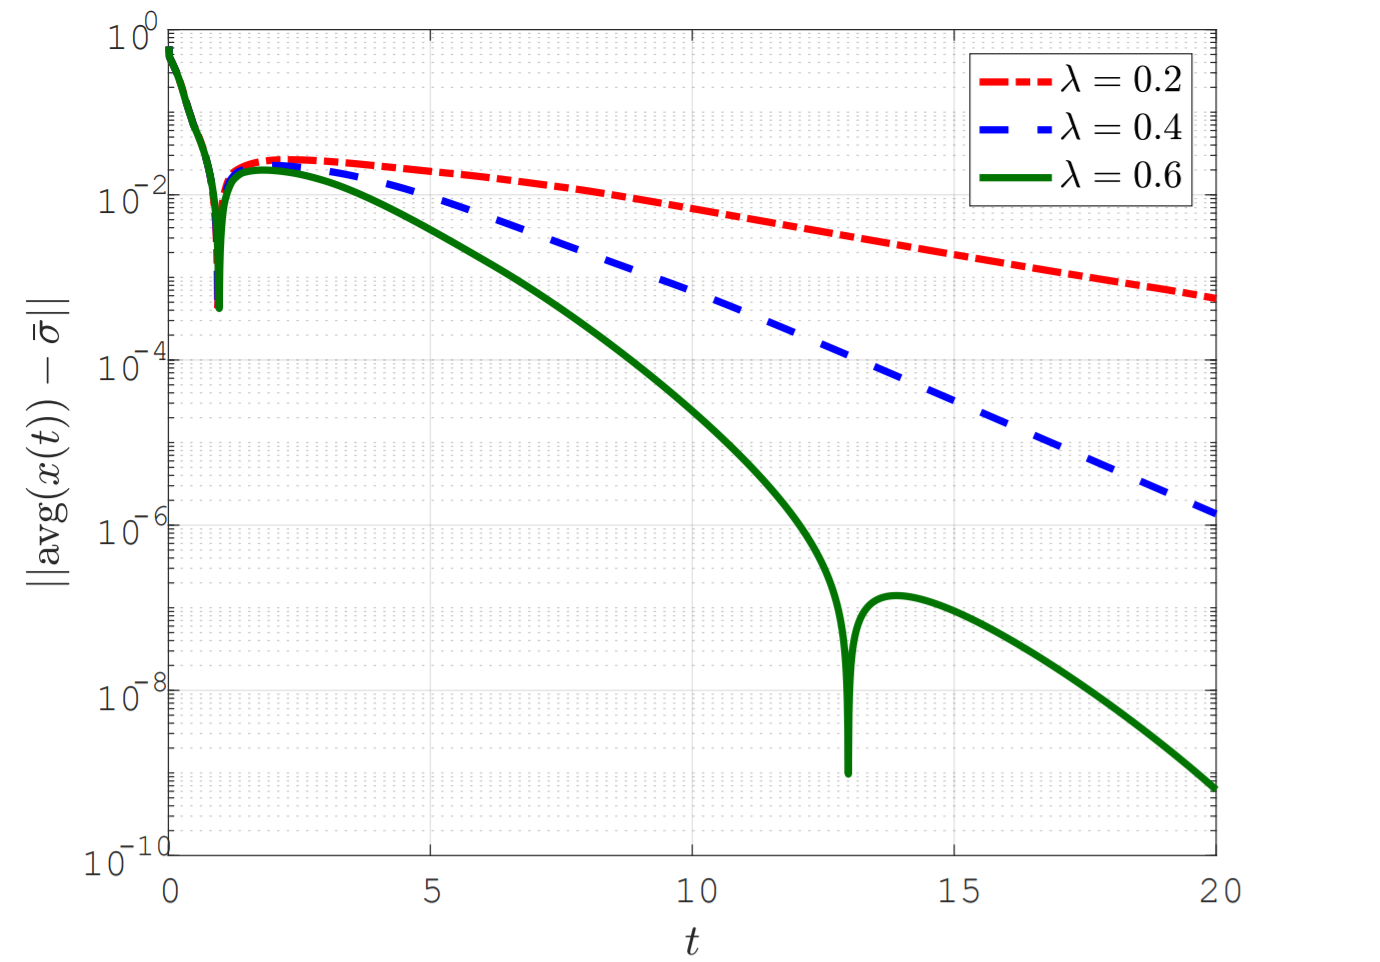
\includegraphics[scale=0.5]{plot11.png}}
\caption{Відстань між середніми стратегіями досліду та рівноваги.}
\label{ris:plot11}
\end{figure}

\subsubsection*{Алгоритм}
З метою досягнення рівноваги пропонується скористатись неперервною динамікою часу:
\begin{align}
\dot x_i &= \prod_{X_i}\left(x_i, -\partial g_i(x_i)-C\sigma\right), \quad \forall i \in N\\
\dot \sigma &= \lambda\left(-\sigma+\mathbf{\bar{x}}\right)\label{lambda} 
\end{align}
де
\begin{equation}
\partial g(x) = \left\{ v \in \mathbb{R}^m~|~g(z)\geq g(x)+v^\mathrm{T}(z-x),\forall z \in \left\{x\in \mathbb{R}^m~|~g(x)< \infty\right\}\right\}
\end{equation}
субдиференціальний набір значень, якщо $g$ диференційована по $x$, то $\partial g(x) = \{\nabla g(x)\}$, та $\lambda>0$ вільний параметр.  

Зазначимо, що структура обчислень та обміну інформацією є напівдецентралізованою: гравці виконують обчислення і не обмінюються інформацією між собою, в той час, як центральний блок управління, який не бере участі в грі, збирає середнє значення їх рішень $\mathbf{\bar{x}}(t)$ та передає сигнал $\sigma(t)$ гравцям.

\begin{figure}[]
\center{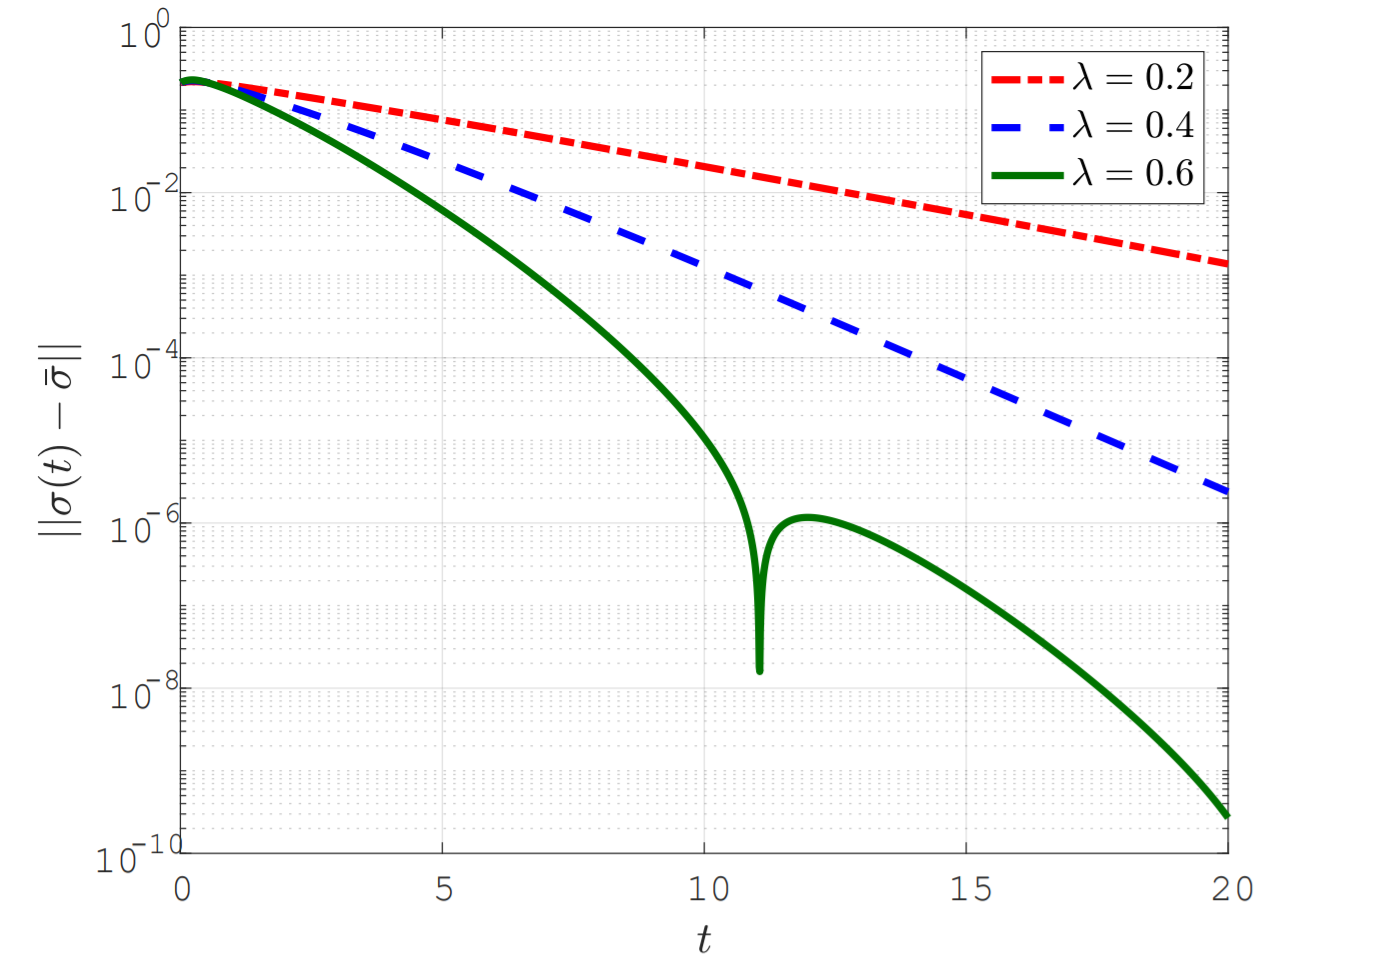
\includegraphics[scale=0.5]{plot22.png}}
\caption{Відстань між інтегральним керуючим сигналом та його рівновагою.}
\label{ris:plot22}
\end{figure}

\subsubsection*{Числове моделювання}
Одною з основних областей застосування агрегатних ігор є
управління попитом, де гравці є споживачами або виробниками електроенергії, чия функція витрат залежить від середнього показника попиту електроенергії, через загальну ціну на неї. Наприклад, у [\ref{Cite22}, розділ 5.2], функція індивідуальних витрат кожного гравця обирається як:
\begin{equation}
    f_i(x_i,\sigma)=\frac{1}{2}l_i\|x_i-x_i^*\|^2+(a\sigma+b)^\mathrm{T}x_i~,
\end{equation}
де $x_i^* \in \mathbb{R}$ досяжна змінна, параметр $l_i>0$, параметри $a \in \mathbb{R}$ та $b \in \mathbb{R}^n$.

Для досліду були взяті наступні значення параметрів: $N=100, a=1,\\ b=0.5, X_i=[0.25, 0.75], x_i^* \sim U(0,1)$ та $l_i = 1.5, ~\forall i\in N$.

Розглянуто задачі для трьох випадків $\lambda=0.2, \lambda=0.4, \lambda=0.6$, графіки ілюструють відстань між середньою стратегією досліду та середньою стратегією рівноваги в часі $\|\mathbf{\bar{x}}(t) - \bar{\sigma}\|$ (Рис.\ref{ris:plot11}), а також відстань між інтегральним керуючим сигналом $\sigma(t)$ та його рівновагою $\bar{\sigma}$ (Рис.\ref{ris:plot22}).

Згідно з попередніми дослідженнями коефіцієнт посилення $\lambda$ з (\ref{lambda}) може помітно пришвидшити зближення до рівноваги, але тільки до критичного значення, вище якого можуть виникати коливання.
\subsubsection*{Висновок}
В контексті агрегатних ігор, інтегральна динаміка з неперервним часом, напівдецентралізованими обчисленнями та обміном інформацією може забезпечити глобальну асимптотичну збіжність до агрегатних рівноваг за умови посилення контролю обраного належним чином. Майбутні дослідження будуть зосереджені на розширенні збіжності та аналізі на випадок загальних мережевих ігор, можливо, з обмеженням та різними технічними припущеннями.

\clearpage
\subsection{Лінійно збіжний алгоритм \cite{Article2}}
Новий розподілений алгоритм спільно використовує ідеї алгоритму консенсусу та умовного проєкційного спуску \cite{Cite1}. За сильно монотонного припущення про псевдоградієнтне відображення, доведемо запропонований алгоритм із фіксованими розмірами кроків, що лінійно збігається до рівноваги Неша. Потім теоретичні результати перевіримо числовими експерименти.

\subsubsection*{Мережева агрегативна гра}
Розглянемо набір з $n$ гравців, проіндексованих як $N = \{1, 2, ... , n\}$.
В агрегативній грі функція витрат гравця $i$, $f_i (\mathbf{x}_i
, \mathbf{\bar{x}})$ залежить від власної дії $\mathbf{x}_i \in X_i \subset \mathbb{R}^p$ та сукупності дій гравців $\mathbf{\bar{x}} = \frac{1}{n} \sum_{i=1}^{n} \mathbf{x}_i$ . Завдання гравця $i$ в АГ полягає в мінімізації його витрат: $f_i (\mathbf{x}_i, \mathbf{\bar{x}})$ де $\quad\mathbf{x}_i \in X_i$, a $ \mathbf{x}_j$, $j \neq i$, $j \in N$ фіксовані, та пошук рівноваги Неша відбувається для всіх гравців.
Взаємодія гравців між собою описується матрицею ваг $W = \{w_{ij}\}_{n\times n}$ де $w_{ij} > 0$ якщо гравці спілкуються, та $w_{ij} = 0$ в іншому випадку.
\subsubsection*{Алгоритм}
Спочатку для кожного гравця $i \in N$ обираємо стратегію $\mathbf{x}_i^0 \in X_i$ випадковим чином та $\mathbf{v}_i^0=\mathbf{x}_i^0$.

Повторюємо наступну процедуру для всіх гравців $i \in N$ допоки не зійдемось. 
\begin{align}
\mathbf{\hat{v}}^{k+1}_i &= \sum_{j=1}^{n} w_{ij}\mathbf{v}^k_j,\\
\mathbf{\hat{x}}^{k+1}_i &= \prod_{X_i} \left[\mathbf{x_i^k-\alpha F_i\left(\mathbf{x_i^k},\mathbf{\hat{v}}^{k+1}_i\right)}\right],\\
\mathbf{x}^{k+1}_i &= \mathbf{x}^{k}_i + \beta\left(\mathbf{\hat{x}}^{k+1}_i-\mathbf{x}^{k}_i\right),\\
\mathbf{v}^{k+1}_i &= \mathbf{\hat{v}}^{k+1}_i + \mathbf{x}^{k+1}_i-\mathbf{x}^{k}_i.
\end{align}
де $\alpha$ оберемо достатньо малим, щоб послідовність $\{\mathbf{x}^k\}_{k\in \mathbb{N}}$ збігалась до фіксованої точки $\mathbf{x}^*$, $\mathbf{v}_i$ локальний вектор, що змінюється в залежності від дій сусідів, $\alpha > 0$ та $\beta \in (0,1]$ розмір кроку.

\begin{figure}[]
\center{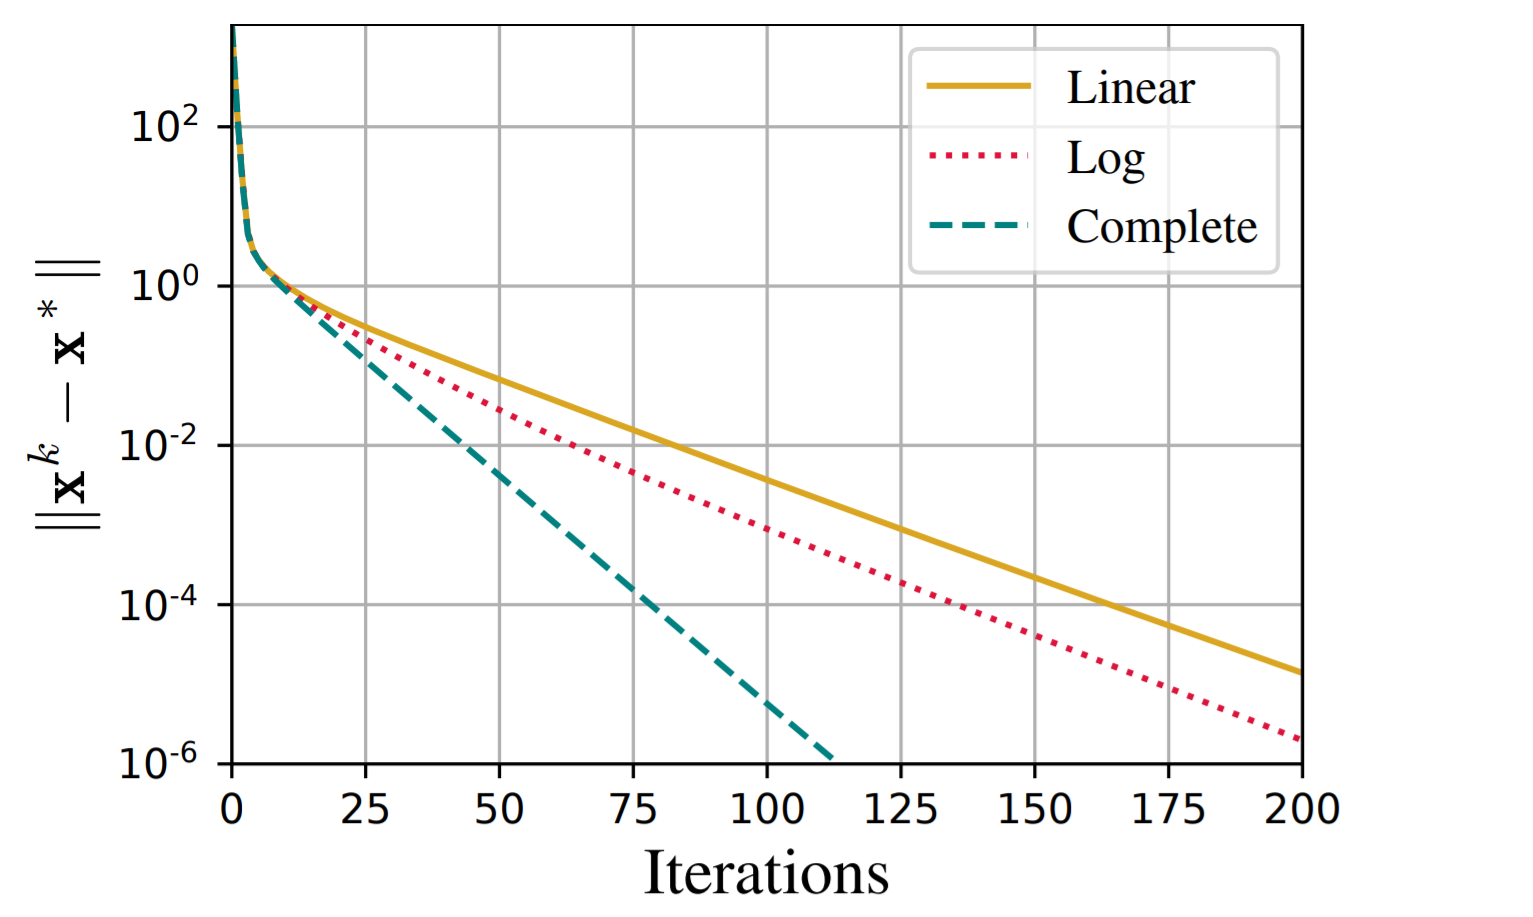
\includegraphics[scale=0.4]{plot1.png}}
\caption{Траєкторії розриву субоптимальності у різних топологіях мережі.}
\label{ris:plot1}
\end{figure}

\subsubsection*{Числовий експеримент}
Розглянемо $n = 20$ фірм, що контролюють $L = 10$ локацій, кожній фірмі $i$ потрібно обрати її продукцію $g_{il}$, та знижки $s_{il}$ на локації $l$.

Ціну продукції фірми $i$ на локації $l$ позначимо як $c_{il}(g_{il})$ та визначимо як
$c_{il}(g_{il}) = a_{il}g_{il} + b_{il}g_{il}^2,$ де $a_{il}$ та $b_{il}$ параметри фірми $i$.

Дохід фірми $i$ на локації $l$ є $s_{il}p_{l}(s_l)$ де $s_l = \sum_{i=1}^{n} s_{il}$ загальна знижка локації та $p_{l}$ відповідна функція ціни.

Функція ціни $p_l$ є функцією резервного попиту та визначається як $p_l(s_l) = d_l - s_l,$ де $d_l$ це параметр локації $l$.

Місткість продукції фірми $i$ на локації $l$ запишемо як $cap_{il}$. Припускаючи, що плата за транспортування між двома локаціями нульова, тоді проблема для фірми $i$ виглядає так:
\begin{align}
&\sum_{l=1}^L \left[c_{il}(g_{il}) - s_{il}\cdot p_l(s_l)\right] \rightarrow min\\
&g_{il},s_{il}\geq 0, \quad g_{il} \leq cap_{il},\\
&\sum_{l=1}^L g_{il} = \sum_{l=1}^L s_{il}.
\end{align}
У симуляції було покладено $a_{il} \sim U(2,12), b_{il} \sim U(2,3), d_l \sim U(90,100)$ та $cap_{il} = 500$ для $i = 1, ..., n$ та $l = 1, ..., L.$ де $U(u_1,u_2)$ рівномірний розподіл на інтервалі $[u_1, u_2]$.

Алгоритм було розглянуто для трьох випадків:
\begin{itemize}
\item \textit{Linear}: гравець $i$ спілкується з гравцями mod$(i+11j,n)+1, 0 \leq j < n/11.$
\item \textit{Log}: гравець $i$ спілкується з гравцями mod$(i+2^j,n)+1, 0 \leq j < \mathrm{log}_{2}~n.$
\item \textit{Complete}: кожен гравець спілкується зі всіма.
\end{itemize}

\begin{figure}[]
\center{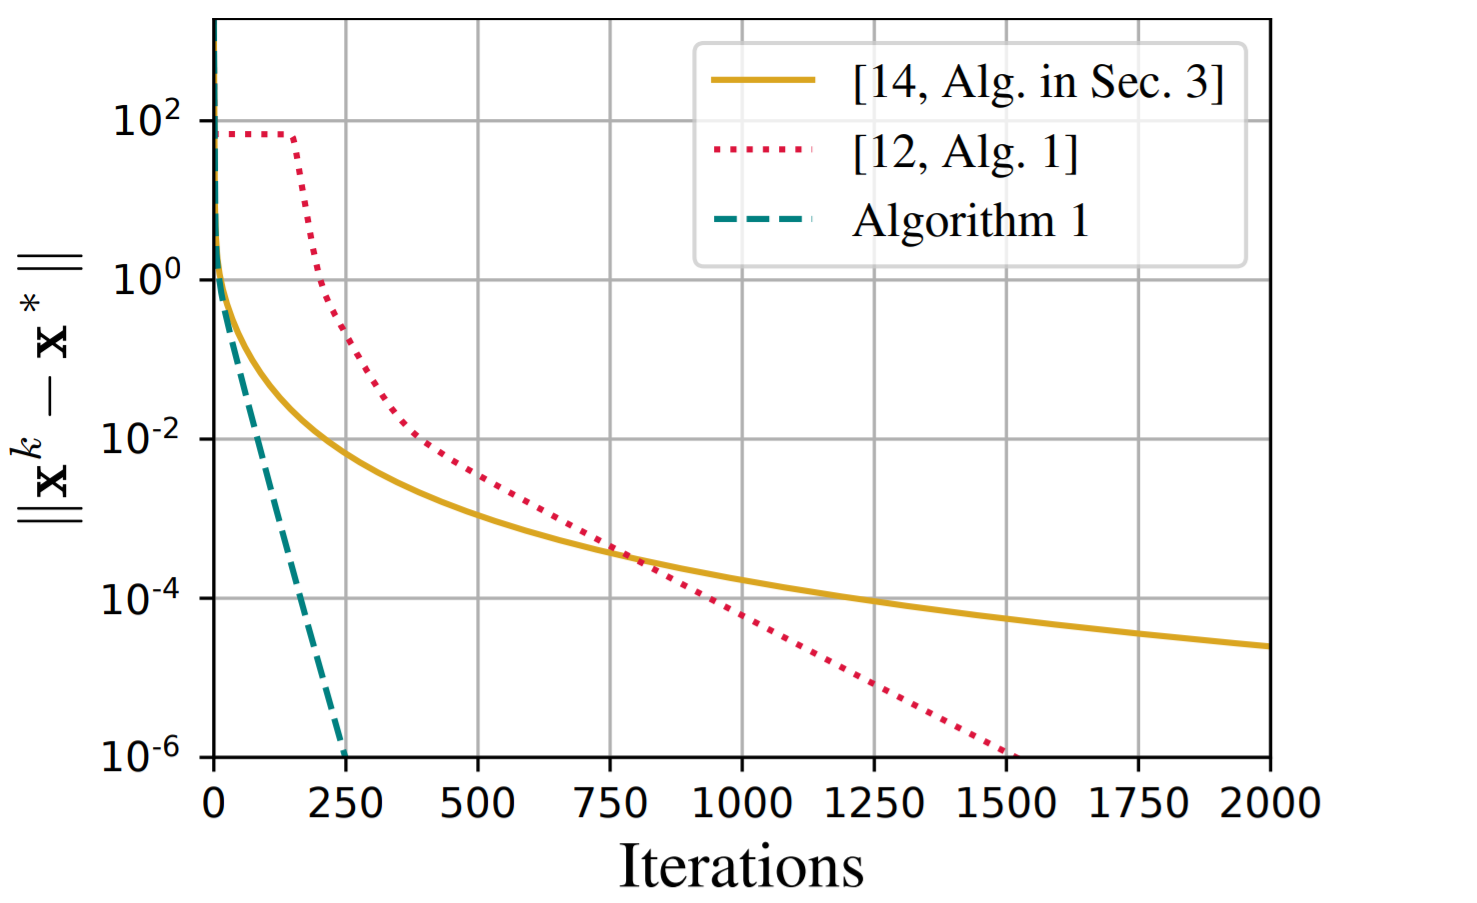
\includegraphics[scale=0.4]{plot2.png}}
\caption{Порівняння різних алгоритмів.}
\label{ris:plot2}
\end{figure}

Матриця ваг $W = \{w_{ij}\}$ задається так
\begin{eqnarray}
w_{ij} =
\begin{cases}
0, & (i,j) \notin E \\
\delta, & (i,j) \in E, i\neq j\\
1-\delta \cdot d(i), &  i = j
\end{cases}
\end{eqnarray}
де $d(i)$ число гравців, що спілкуються с гравцем $i$, та $\delta = 0.5/\mathrm{max}_i{d(i)}$, та $E$ множина пар, що спілкуються між собою. Рис.~\ref{ris:plot1} описує траєкторії субоптимального розриву $||\mathbf{x}^k - \mathbf{x}^*||$ для різної кількості ітерацій, для трьох мережевих топологій. Всі топології починаються з однієї точки з оптимальним розміром кроку. Можна бачити, як алгоритм лінійно збігається для різних топологій.

Щоб знайти оптимальне значення коефіцієнта $\alpha$ фіксуємо різні значення коефіцієнта $\beta$, приклад лінійної топології наведено у таблиці.

\begin{wraptable}{l}{0.65\linewidth}
\begin{tabular}{ | c | c | c | c | c | c | c | }
\hline
$\beta$&& 0.8&0.85 &0.9 &0.95 &1 \\\hline
$\alpha$&&0.108 &0.092 &0.096 &0.090& 0.087\\\hline
$\varepsilon _{200} (\times 10^{-5})$&& 1.615&1.622 & \textbf{1.418}&1.512 &1.591\\
\hline
\end{tabular}
\end{wraptable}
Порівняємо описаний та \cite{Cite2}, \cite{Cite3} алгоритми, з яких перший призначений для ігор, де функції витрат залежать від дій загалом, а останній призначений для мережевої агрегативної гри, але лише зі зменшенням розмірів кроків. Рис.~\ref{ris:plot2} показує, що описаний алгоритм перевершує інші. Алгоритм \cite{Cite2} застряє у початковій фазі, яка обумовлена властивістю кожного гравця робити помилкову оцінку дій сусідів. Що стосується алгоритму в \cite{Cite3}, то він використовує зменшувані розміри кроків та також поступається описаному алгоритму.

\subsubsection*{Висновок}
Вище був запропонований повністю розподілений алгоритм для мережевої агрегативної гри за ненаправленим зв’язком мережі. Коли мережева агрегативна гра є сильно монотонною та має безперервне псевдоградієнтне відображення Ліпшіца. Доведено, що алгоритм з фіксованими розмірами кроків збігається лінійно до унікальної рівноваги Неша. Теоретичні результати були підтверджені числовими експериментами. У подальшій роботі будуть розглянуті лінійно збіжні алгоритми для мережевих агрегативних ігор через мережі спрямованого зв'язку або мережі, що змінюються з часом.
\clearpage
\section{Дослідження}
У реальному житті вибір людей залежить від багатьох факторів, що заважають обрати найкращу стратегію, не кажучи вже про те, що деякі люди не можуть взагалі раціонально мислити. Тому я вирішив провести власне дослідження та проаналізувати його результати.

Дослідження являє собою опитування громадської думки у розмірі ста осіб, слід зазначити, що я не володію ресурсами для масового опитування громадян, на відміну від деяких маркетингових компаній, тому висновки даного дослідження не можна проєктувати на всіх людей, та вважати істиною в останній інстанції. Значна частина учасників дослідження становлять студенти технічних спеціальностей, декілька з біологічних та лінгвістичних, та пара людей середнього віку.

Опитування має у собі три гри, а саме: \textit{«Дилему в'язня»} п.~\ref{prison}, \textit{«Гарвард»} п.~\ref{garvard}, \textit{«Вгадай число»} п.~\ref{smallest}. 

\subsection{Дилема в'язня}
\begin{figure}[h]
\center{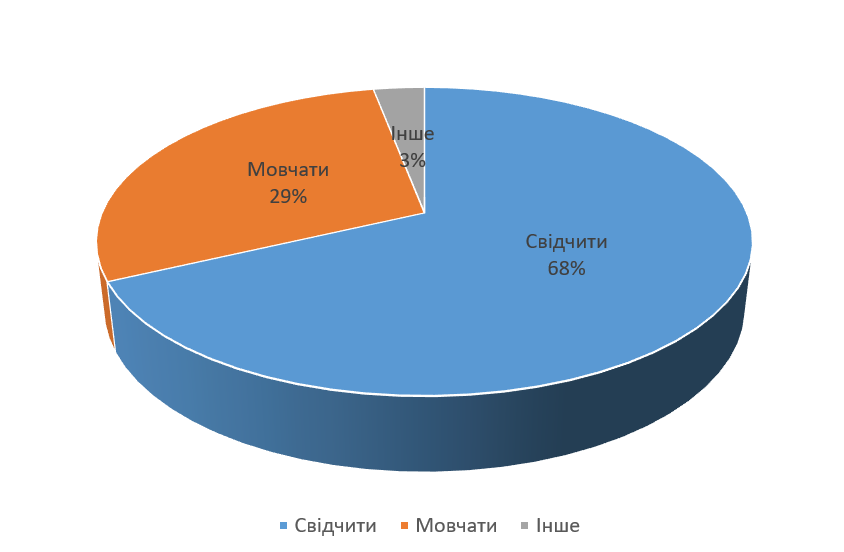
\includegraphics[scale=0.7]{prison.png}}
\label{ris:prison}
\end{figure}

Нагадаємо, що \textit{«Дилема в'язня»} п.~\ref{prison} полягає у тому щоб обрати між зрадою та мовчанням стосовно свого товариша, з точки зору моралі звісно потрібно мовчати, але у реальному житті люди надають перевагу своїм інтересам більше ніж інтересам інших.

Якщо подивитись з боку тих мовчить, вони напевно вважають, що більшість людей є такими \textit{<<раціональними агентами>>}, та стратегія \textit{<<мовчати>>} принесе більше користі ніж інша. Але дослідження показує, що якщо все-таки обрати цей варіант, то лише майже у \textbf{30\%} випадків ми отримаємо пів року ув'язнення, а у \textbf{70\%} десять років. Апріорне математичне сподівання такого вибору буде приблизно $0.298\cdot0,5+0.702\cdot10 =$ \textbf{7.16 років}, що на мою думку не є бажаним результатом.

З іншого боку люди, що обирають стратегію \textit{<<свідчити>>}, мають апріорне математичне сподівання $0.298\cdot0+0.702\cdot2 =$ \textbf{1.4 років}, що все ж таки більше за пів року в ідеальному випадку, але не на багато.

Будь-яка змішана стратегія стосовно нашого випадку буде давати математичне сподівання між \textbf{1.4} та \textbf{7.16 років}, тому її не варто розглядати, достатньо лише обмежитись чистими стратегіями для висновку.

\textbf{Отже,} у суспільстві для досягнення власної вигоди потрібно дотримуватись стратегії \textit{<<свідчити>>}. Добре це чи ні? Нехай відповідь на це питання кожен визначить самостійно.

\subsubsection*{Коментарі}
\begin{itemize}
\item \textit{<<Якщо впевнена, що інший підозрюваний не буде свідчити проти мене, то \textbf{мовчати}, якщо є великі сумніви в ньому, то \textbf{свідчити}, а якщо не впевнена просто в ньому, то \textbf{свідчити} бо хто знає, що йому там в голову може прийти)))>>}

\item \textit{<<\textbf{Мовчати} (довіра — валюта економіки, хоча і немає рівноваги Неша)>>}
\item \textit{<<\textbf{Мовчати}, адже строк буде меншим, проте залежить від того наскільки добре я знаю іншу людину>>}
\item \textit{<<Перший раз \textbf{мовчати}, а далі робити так, як робив інший на попередньому кроці. Найефективніша стратегія :)>>}
\item \textit{<<Я б \textbf{мовчав} бо братанів здавати не можна. І ще питання чого мене засудять на 6 місяців якщо сказано що немає доказів?>>}

\item \textit{<<Мовчати доволі ризиковано, оскільки можна влетіти на 10 років. Краще \textbf{свідчити}, тоді або ти відразу вільний, або 2 роки.>>}
\item \textit{<<Потрібно \textbf{свідчити}, якщо в'язням відома система, треба доносити один на одного, домовившись раніше за арешт.>>}
\item \textit{<<\textbf{Свідчити}, тоді незалежно від того, що обере другий, я зроблю краще для себе>>}
\item \textit{<<\textbf{Свідчити}, якщо попередньо не домовлялися мовчати. Якщо домовлялися — \textbf{мовчати}>>}
\item \textit{<<\textbf{Засвідчу.} Найвигіднішим вибором є мовчати, але інший підозрюваний з більшою ймовірністю також буде свідчити.>>}
\item \textit{<<Конечно \textbf{предать}, это выгодно для тебя, и рационально, нерациональные ходы направленные на кооперацию могут привести к нерациональному решению против самого тебя.>>}
\end{itemize}

\subsection{Гарвард}
\begin{figure}[h]
\center{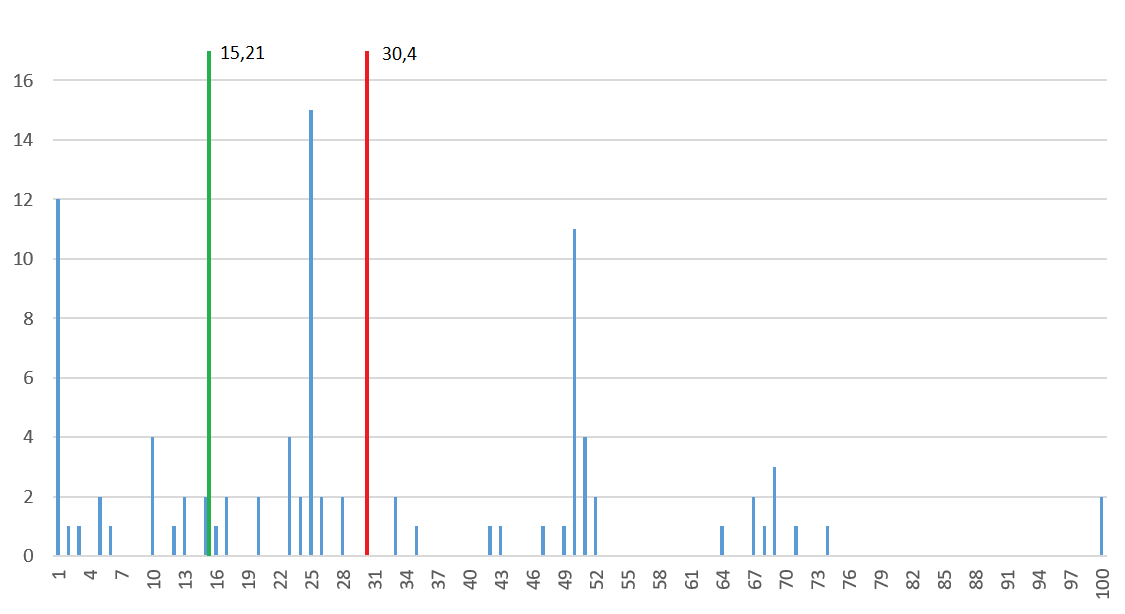
\includegraphics[scale=0.63]{garvard.png}}
\end{figure}
\textit{<<Гарвард>>} п.~\ref{garvard} — гравці обирають числа від 1 до 100, виграє той чиє число буде ближче до половини середнього арифметичного.

У ідеальному варіанті, що описується у п.~\ref{garvard}, всі учасники повинні були обрати 1 та виграти, але на жаль реальний світ не є ідеальним. Кожен обирав те що хотів та здобули перемогу люди, що обрали число \textbf{15}.

Правильний хід думок було висловлено у першому коментарі до цієї задачі, отже я не буду їх повторювати.

Але потрібно зазначити, що деякі учасники неправильно зрозуміли умову й обирали числа 50 та 51 оскільки вважали, що вони є \textit{<<найближчі до середнього>>}. Якщо відкинути цей факт, все одно залишається менша частина людей, що обирали числа у правій частині відрізка з незрозумілих, як на мене, причин.

Розподіл отриманий під час дослідження цієї задачі нагадує суміш нормальних розподілів з математичними сподіваннями 1, 25, 50, 70.

Люди самі по собі не є раціональними, але я сподіваюсь що це не спричинить шкоди у більш важливих сферах ніж ігри.

\subsubsection*{Коментарі}
\begin{itemize}
    \item \textit{<<Цікаво дослідити рівномірний розподіл у другій задачі серед людей, оскільки потрібно вибрати таке число аби воно було близьке до половини середнього арифметичного, це означає, що спочатку кожне число від 1 до 100 буде поділено на 2, отже інтервал зменшиться до від 1 до 50, звідси одразу стає зрозуміло, що обирати числа від 50 до 100 ірраціонально. Далі цікаво дослідити розподіл серед 1 до 50. Якщо спиратись на розподіл Ґауса, то визначимо, що скоріш за все люди оберуть число близьке до середини, тобто 25, але якщо прийняти той факт, що дехто буде обирати числа по типу 60 чи 70 то скоріш треба обрати 26-27.>>}
%    \item \textit{<<Друге завдання чисто статистичне, але опитування досить таке ультрарозумне.>>}
    \item \textit{<<Извините, меня из уника выгнали>>}
\end{itemize}

\subsection{Вгадай число}
\begin{figure}[h]
\center{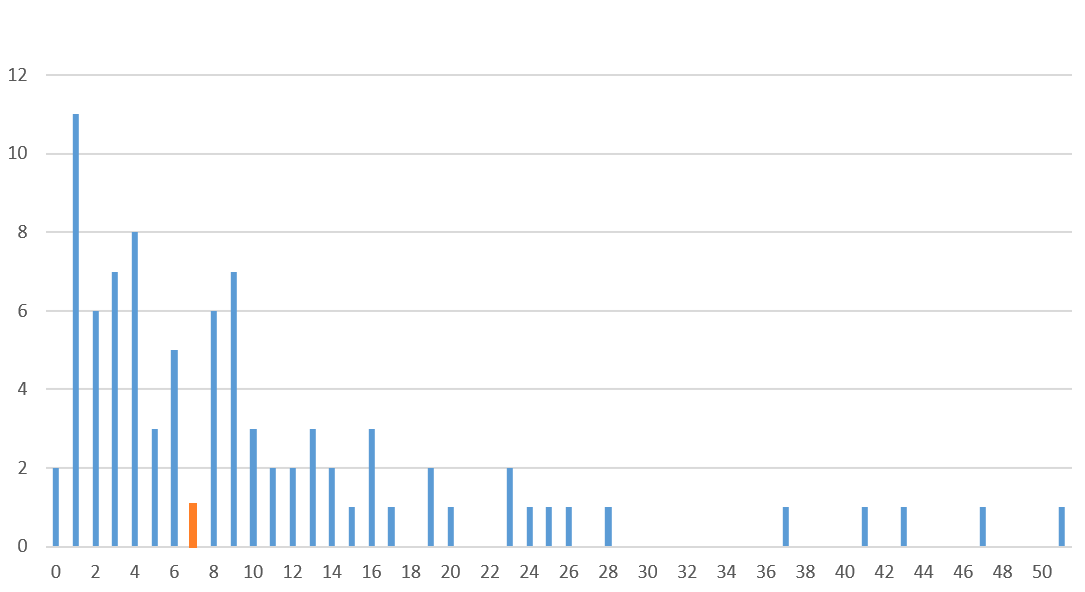
\includegraphics[scale=0.76]{smallest.png}}
\label{ris:smallest}
\end{figure}

\textit{<<Вгадай число>>} п.~\ref{smallest} — потрібно обрати найменше ціле невід'ємне число, яке ніхто інший не обрав.

Число-переможець — \textbf{7}, цікаво, що отримана ситуація є рівновагою Неша та була описана у третьому прикладі п.~\ref{smallest}.

Зазвичай у подібних іграх гравці знають загальну кількість учасників, але на жаль як я, так і вони, у цій грі його не знали. Цей факт обмежує варіанти для роздумів, та змушує робити додаткові припущення, але, як на мене, не є критичним.

Розподіл отриманий у даній грі нагадує логнормальний $\ln N\left(0 , \left(\frac{3}{2}\right)^{2}\right)$, але як вже було сказано вибірка є занадто маленькою, щоб висувати якісь гіпотези з цього приводу.


\subsubsection*{Коментарі}
\begin{itemize}
    \item \textit{<<Найважче було підібрати дисперсію для нормального розподілу для задачі №3, звісно такий метод не виключає випадкових відповідей типу як \textbf{"оберу улюблене число"}, але мені здається, що люди, які зрозуміли умову задачі, не будуть думати в термінах \textbf{"гороскопів"}.>>}
    \item \textit{<<Гравці мають знати кількість своїх противників.>>}
    \item \textit{<<*тут мозок зламався* $7$>>}
\end{itemize}

\clearpage
\section{Висновки}

На закінчення слід особливо підкреслити, що теорія ігор є дуже складною сферою знань. При поводженні з нею треба дотримуватися правил та бути дуже обережним, чітко знати межі її застосування. Аналіз і консультації на основі теорії ігор через їх складності рекомендуються лише для особливо важливих проблемних областей. Однак застосування теорії ігор полегшує нам розуміння суті того, що відбувається, а багатогранність даного розділу науки дозволяє нам успішно використовувати методи й властивості цієї теорії в різних областях нашої діяльності.

Теорія ігор прищеплює людині дисципліну розуму. Від особи, яка приймає рішення, вона вимагає систематичного формулювання можливих альтернатив поведінки, оцінки їх результатів, і найголовніше — дослідження поведінки інших. Людина, знайома з теорією ігор, рідше вважає інших дурнішими за себе, і тому уникає багатьох непробачних помилок. Однак теорія ігор не може, та й не розрахована на те, щоб надати рішучості, наполегливості в досягненні цілей, всупереч невизначеності та ризику. Знання основ теорії ігор не дає нам явного виграшу, але оберігає нас від звершення дурних і непотрібних помилок.

В останні роки значення теорії ігор істотно зросло в багатьох областях економічних і соціальних наук. В економіці вона застосовна не тільки для вирішення загальногосподарських завдань, а й для аналізу стратегічних проблем підприємств, розробок організаційних структур і систем стимулювання.

В умовах альтернативи дуже часто нелегко прийняти рішення і вибрати ту чи іншу стратегію. Дослідження операцій дозволяє за допомогою використання відповідних математичних методів прийняти обґрунтоване рішення про доцільність тієї чи іншої стратегії. Теорія ігор, що має в запасі арсенал методів вирішення матричних ігор, дозволяє ефективно вирішувати зазначені завдання декількома методами й з їх безлічі вибрати найбільш ефективні.

На закінчення можна зробити висновок про необхідність використання теорії ігор в сучасності.

Дисципліна створена для математичного вирішення завдань економічного і соціального походження, не може в цілому зводитися до класичних математичних теорій, створених для вирішення фізичних і технічних завдань. Однак в різних конкретних питаннях теорія ігор широко використовує різноманітні класичні математичні методи. Крім цього, вона пов'язана з рядом математичних дисциплін внутрішнім чином. У теорії ігор систематично і по суті вживаються поняття теорії ймовірностей. Її мовою можна сформулювати більшість завдань математичної статистики.

У даній роботі я намагався донести основні поняття теорії ігор, історію створення цієї дисципліни, подальше вивчення якої потребує великого бажання та впевненості у тому, що сили витрачені на це не будуть занадто великі у порівнянні з отриманим результатом. Якщо ви хочете обрати теорію ігор своєю справою, спочатку добре подумайте, перед тим як робити такий вибір.

\clearpage
\section{Словник термінів}

\textbf{Агрегативна гра} — це гра, в якій виграш кожного гравця є функцією власної стратегії гравця та сукупності стратегій усіх гравців.

\textbf{Аксіома вибору} — аксіома теорії множин, яка еквівалентна твердженню, що декартів добуток колекції непорожніх множин є також не порожнім.

\textbf{Альтернатива} — необхідність вибору однієї з двох можливостей, що виключають одна одну.

\textbf{Апріорна ймовірність} —  це розподіл ймовірності, що виражатиме чиєсь переконання про деяку подію перед врахуванням якогось свідчення.

\textbf{Безперервна гра} — гра, що продовжуються нескінченну кількість часу.

\textbf{Гра} — взаємодія гравців, що мають певні можливості діяти, та отримують виграш під кінець гри.

\textbf{Гра біматрична} — безкоаліційна гра двох гравців, яка має скінченну кількість стратегій.

\textbf{Гра з кінцевою кількістю кроків} — повна протилежність, вони обмежені кількістю їх.

\textbf{Гра з ненульовою сумою} — виграш одного гравця не означає програш іншого.

\textbf{Гра з неповною інформацією} — гравці мають у своєму розпорядженні лише частковою інформацією про ворога.

\textbf{Гра з нескінченним числом кроків} — не має обмеження в кількості кроків.

\textbf{Гра з нульовою сумою} — гра з постійним фондом гри, доступні ресурси гри не можуть стати більше або менше.

\textbf{Гра з повною інформацією} — учасники знають всі ходи, зроблені до поточного моменту, так само як і можливі стратегії супротивників. 

\textbf{Гра у нормальній формі} — описує статичну взаємодію гравців, не передбачаючи можливості послідовних ходів, накопичення інформації про дії суперника та повторюваної взаємодії.

\textbf{Гібридна гра} — кожен гравець буде переслідувати інтереси своєї групи та водночас спробувати отримати особистий прибуток.

\textbf{Дискретна гра} — гра з обмеженою кількістю кроків, подій, результатів.

\textbf{Дисперсія} — це міра розсіяння значень випадкової величини відносно середнього значення розподілу.

\textbf{Домінантна стратегія} — стратегія, що дає більший виграш, ніж інша, при будь—яких діях опонентів гравця.

\textbf{Домінантний розв'язок} — ситуація при якій у кожного гравця є домінантна стратегія.

\textbf{Досконала конкуренція} — ідеалізований стан ринку (ідеальна ринкова структура), коли окремі покупці й продавці не можуть впливати на ціну.

\textbf{Дослідження операцій} — це дисципліна, що займається розробкою й застосуванням методів знаходження оптимальних рішень на основі математичного моделювання у різних областях людської діяльності.

\textbf{Змішана стратегія} — стратегія, яка полягає в тому, що гравець застосовує одну зі своїх чистих стратегій, обрану в кожній грі за випадковим законом.

\textbf{Кібернетика} — наука про загальні принципи керування в комплексі складними системами різної природи походження.

\textbf{Класична дилема в’язня} — гра з ненульовою сумою, в якій гравці прагнуть одержати вигоду, співпрацюючи один з одним або зраджуючи.

\textbf{Конвергенція} — економічне зближення двох або кількох суб'єктів господарювання, регіонів або країн.

\textbf{Конкурентна економіка} — це економічний процес взаємодії й боротьби товаровиробників за найвигідніші умови виробництва і збуту товарів, за отримання найбільших прибутків.

\textbf{Конкурентна рівновага} — це умова, при якій виробники, що максимізують прибуток, та споживачі, що максимізують корисність, на конкурентних ринках із вільно визначеними цінами досягають рівноважної ціни. При цій рівноважній ціні поставлена кількість дорівнює необхідній кількості.

\textbf{Конфлікт} — зіткнення протилежних інтересів і поглядів, напруження і крайнє загострення суперечностей, що призводить до активних дій, ускладнень, боротьби, що супроводжуються складними колізіями; ситуація, в якій кожна зі сторін намагається зайняти позицію несумісну з інтересами іншої сторони.

\textbf{Кооперативна гра} — гравці можуть об'єднуватися в групи, брати на себе зобов'язання перед іншими гравцями й координувати свої дії.

\textbf{Логнормальний розподіл} — двопараметричне сімейство абсолютно неперервних розподілів. Якщо випадкова величина має логнормальний розподіл, то її логарифм має нормальний розподіл.

\textbf{Модель Бертрана} — модель цінової конкуренції на олігополістичному ринку, сформульована французьким математиком і економістом Жозефом Бертраном у 1883 році.

\textbf{Модель поведінки} — стратегія або стратегії якими володіє гравець.

\textbf{Монографія} — наукова праця у вигляді книги з поглибленим вивченням однієї або кількох тем.

\textbf{Некооперативна гра} — в теорії ігор, гра в якій гравці приймають рішення незалежно один від одного.

\textbf{Несиметрична гра} — гравці матимуть різні винагороди.

\textbf{Нормальний розподіл (розподіл Ґауса)} — розподіл ймовірностей випадкової величини, що характеризується густиною ймовірності.

\textbf{Олігополії} — структура ринку, при якій в одній галузі домінує невелика кількість конкурентних фірм, при цьому хоча б одна або дві з них, виробляють значну частку продукції даної галузі, а поява нових продавців ускладнена чи неможлива.

\textbf{Оптимальна стратегія} — стратегія гравця у якій він гарантує собі виграш, не менший, ніж значення гри, незалежно від вибору стратегії суперником.

\textbf{Паралельна гра} — всі гравці можуть зробити дію в даний відрізок часу.

\textbf{Парето—оптимум} — економічний термін, який описує такий стан системи, при якому значення кожного окремого критерію, що описує стан системи, не може бути покращено без погіршення становища інших елементів.

\textbf{Послідовна гра} — учасники можуть робити ходи в заздалегідь встановленому або випадковому порядку, але при цьому вони отримують деяку інформацію про попередніх діях інших.

\textbf{Рівновага Неша} — сукупність стратегій або дій, згідно з якими кожен учасник реалізує оптимальну стратегію, передбачаючи дії суперників.

\textbf{Рівномірний розподіл} — в теорії імовірностей розподіл, який характеризується тим, що ймовірність будь-якого інтервалу залежить тільки від його довжини.

\textbf{Середнє арифметичне} — сума всіх фіксованих значень набору, поділена на кількість елементів набору.

\textbf{Симетрична гра} — це гра, коли виграш, за відтворення певної стратегії, залежить лише від наступних стратегій, а не від того, хто в ній грає.

\textbf{Симплекс} — геометрична фігура, що є багатовимірним узагальненням трикутника і тетраедра. 

\textbf{Ситуація гри} — набір стратегій, обраних усіма гравцями.

\textbf{Спектральний радіус матриці} — максимум модуля її власних значень.

\textbf{Стратегія} —  це загальний, недеталізований план, що охоплює довготривалий проміжок часу, спосіб досягнення важливої мети.

\textbf{Теорія дослідження операцій} — це дисципліна, що займається розробкою й застосуванням методів знаходження оптимальних рішень на основі математичного моделювання у різних областях людської діяльності.

\textbf{Теорія ігор} — теорія математичних моделей прийняття оптимальних рішень в умовах конфлікту.

\textbf{Теорія ймовірностей} — розділ математики, що вивчає закономірності випадкових явищ: випадкові події, випадкові величини, їхні функції, властивості й операції над ними.

\textbf{Теорія множин} — розділ математики, в якому вивчаються загальні властивості множин.

\textbf{Теорія рішень} — царина досліджень, яка математичними методами досліджує закономірності людського вибору найвигідніших із можливих альтернатив і має застосування в економіці, менеджменті, когнітивній психології, інформатиці та обчислювальній техніці.

\textbf{Функція реакції} — прогноз ймовірного обсягу продажів протягом певного відрізка часу при різних рівнях витрат на один або кілька елементів комплексу маркетингу.

\textbf{Чиста стратегія} — будь-яка із доступних для гравця дій, передбачених правилами гри.

\clearpage
\begin{thebibliography}{05}
\addcontentsline{toc}{section}{\refname}
{\small

\bibitem{Gubko} Губко~М., Новиков~Д. Теория игр в управлении организационными системами, М: Синтег, 2002~г.

\bibitem{Danilov} Данилов~В.~И., Лекции по теории игр. М.: препринт РЭШ, 2002

\bibitem{Zaharov} Захаров~А.~В. Теория игр в общественных науках. М.: препринт НИУ ВШЭ, 2014

\bibitem{Mazalov} Мазалов~В. Математическая теория игр и приложения, Санкт—Петербург, Лань, 2010~г.

\bibitem{Menshikov} Меньшиков~И. Лекции по теории игр и экономическому моделированию, М.: Контакт Плюс 2010~г.

\bibitem{Shen} А.~Шень — Игры и стратегии с точки зрения математики. Москва
Издательство МЦНМО 2018

\bibitem{Neyman} фон~Нейман~Дж., Моргенштерн~Э. Теория игр и экономическое поведение. — М. : Наука, 1970. — 708~с.

\bibitem{Osborne} M.~Osborne and A.~Rubinstein, A Course in Game Theory, MIT press, Cambridge, MA, 1994.

\bibitem{Nesh} Джон Форбс Неш [Електронний ресурс]: Вікіпедія. Вільна енциклопедія.

URL: \url{https://en.wikipedia.org/wiki/John_Forbes_Nash_Jr.}

\bibitem{GameTeory} Теорія ігор [Електронний ресурс]: Вікіпедія. Вільна енциклопедія.

URL: \url{https://en.wikipedia.org/wiki/Game_theory}

\bibitem{GTCourseraSav} Теория игр, МФТИ, Савватеев~А.~В. [Електронний ресурс]: Coursera

URL: \url{https://www.coursera.org/learn/gametheory}

\bibitem{Cite2} M. Bianchi and S. Grammatico, “Fully distributed nash equilibrium seeking over time-varying communication networks with linear convergence rate,” IEEE Control Systems Letters, vol. 5, no. 2, pp. 499–504, 2021.

\bibitem{Cite22}\label{Cite22} S.~Liang, P.~Yi, and Y.~Hong, “Distributed Nash equilibrium seeking for aggregative games with coupled constraints,” Automatica, vol. 85, pp. 179–185, 2017.

\bibitem{Cite3} J. Koshal, A. Nedic, and U. V. Shanbhag, “Distributed algorithms for aggregative games on graphs,” Operations Research, vol. 64, no. 3, pp. 680–704, 2016.

\bibitem{Cite21} C.~De~Persis, S.~Grammatico, “Distributed Nash equilibrium seeking by a consensus based approach,” IEEE Trans. on Automatic Control, vol. 62, no. 9, pp. 4811–4818, 2017.

\bibitem{Article1} C.~De~Persis, S.~Grammatico <<Continuous-time integral dynamics for aggregative game equilibrium seeking>> [Електронний ресурс]: arXiv preprint arXiv:1803.10448v1, 2018

URL: \url{https://arxiv.org/pdf/1803.10448.pdf}

\bibitem{Cite1} R.~Zhu, J.~Zhang, K.~You, and T.~Basar, “Asynchronous networked
aggregative games” [Електронний ресурс]: arXiv preprint arXiv:2101.08973, 2021.

URL: \url{https://arxiv.org/pdf/2101.08973.pdf}

\bibitem{Article2} R.~Zhu, J~Zhang and K~You <<Networked Aggregative Games with Linear Convergence>> [Електронний ресурс]: arXiv preprint arXiv:2105.05465v1, 2021

URL: \url{https://arxiv.org/pdf/2105.05465.pdf}

}
\end{thebibliography}

\end{document}